\subsection{Spark Core}
Spark Core è la base dell'intero progetto: fornisce il dispacciamento distribuito dei compiti, lo scheduling e le funzionalità I/O di base. Spark Core funziona in parte come un livello API. Oltre al motore Spark Core, l’ambiente API Apache Spark viene fornito insieme ad alcune librerie da utilizzare nelle applicazioni di analisi dei dati.
\begin{itemize}
    \item \textbf{Spark SQL}: è un modulo Spark per l'elaborazione di dati strutturati. A differenza delle API di base di Spark RDD, le interfacce fornite da Spark SQL forniscono a Spark più informazioni sulla struttura dei dati e sul calcolo che viene eseguito. Internamente, Spark SQL utilizza queste informazioni extra per eseguire ottimizzazioni. Dato che quando si calcola un risultato, viene utilizzato lo stesso motore di esecuzione, indipendentemente da quale API/linguaggio si sta utilizzando, gli sviluppatori possono facilmente fare avanti e indietro tra diverse API a loro piacimento. DataFrame fa parte di questa libreria.
    \item \textbf{Spark Streaming}: una libreria per l'elaborazione scalabile, ad alta velocità e fault-tolerant di flussi di dati in tempo reale.  I dati possono essere ottenuti da molte fonti come Kafka, Kinesis, o socket TCP, possono essere elaborati tramite algoritmi di Machine Learning ed elaborazione grafica ed infine possono essere inviati a file system, database e dashboard live.
    \item \textbf{MLlib}: una libreria di Machine Learning (ML) il cui scopo è di rendere l'apprendimento automatico facile e scalabile. Essa mette a disposizione algoritmi di Machine Learning, Pipelines e diversi altri strumenti per lo svolgimento di operazioni statistiche avanzate sui dati e per creare applicazioni attorno a queste analisi.
    \item \textbf{GraphX}: è un nuovo componente di Spark per i grafi e il calcolo parallelo su di essi. Per supportare il calcolo dei grafi, GraphX mette a disposizione un insieme di operazioni fondamentali (ad esempio, \textit{subgraph}, \textit{joinVertices}, e \textit{aggregateMessages}). Inoltre, include una crescente collezione di algoritmi e costruttori di grafi per semplificare i compiti di analisi.
\end{itemize}

\begin{figure}[hbt!]
    \centering
    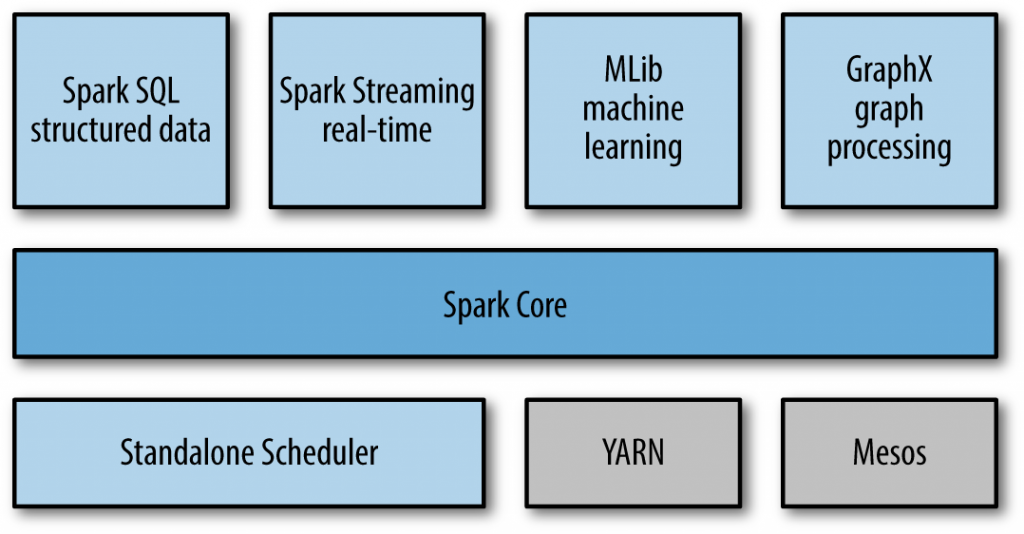
\includegraphics[width=1\textwidth]{img/sparkcore.png}
    \caption{Spark core e librerie}
    \label{fig:spark_core}
\end{figure}
\newpage

